\documentclass[12pt, a4paper]{article}
\usepackage[utf8]{inputenc}
\usepackage[russian]{babel}
\usepackage[T2A]{fontenc}
\usepackage{amsfonts}
\usepackage{amsmath}
\usepackage{indentfirst}
\DeclareMathOperator*{\argmin}{argmin}

\usepackage[left=2cm,right=1.5cm,top=2cm,bottom=2cm]{geometry}
\linespread{1.25}

\usepackage{graphicx}
\graphicspath{{pictures/}}
\DeclareGraphicsExtensions{.pdf,.png,.jpg}

\begin{document}
 \section*{Тема}
Построение оптимального маршрута при заданной модели движения других участников транспортной сети


\section*{Введение}

В данной работе рассматривается задача нахождения наилучшего в каком-то смысле пути с учетом движения фиксированного количества участников по заданным ранее маршрутам в условиях ограниченности модели дорожной системы. Новый построенный маршрут должен отвечать выбранным критериям кратчайшести среди всевозможных путей на всем временном промежутке, но не обязательно в каждый момент времени. Знание маршрутов изначальных участников помогает определить плотность автомобильного потока на конкретных отрезках пути. Рассматриваемая модель приближена к реальной дорожной системе городов, поэтому на всех ее участках наложены ограничения по вместимости участников и скорости их движения. Такие ограничения влияют на показатели маршрутов участников, такие как итоговое время движения и длину пути. 


Тема актуальна в наше время, так как она помогает решить проблему пробок на дорогах, а также призвана упростить водителям выбор маршрута, который займет у них наименьшее время. Задача имеет практический характер... Проблема пробок в Москве стоит очень остро, ученые решают ее не первый год..

В мире прогнозы загруженности используются для автоматического управления дорожным движением в некоторых городах. Первые прототипы, в которых были применены прогнозы, появились появились в 1998 году в США. А первое пилотное использование системы, «заглядывающей в будущее», началось в 2006 году в Сингапуре. Среди наших соотечественников похожей задачей занимается отдел навигации Яндекса. Разработчики собирают информацию по трекам движения автомобилей, осуществляют привязку треков к ребрам графа дорожной сети, вычисляют некоторую усредненную скорость на отдельных участках, рисуют карту прогноза дорожной ситуации на ближайший час и в связи с этим предлагают оптимальный по времени путь, а также еще пару алтернативных маршрутов. Сложность сбора информации и построения треков движения состоит в том, что, во-первых, не все пользуются сервисами Яндекса при построении своего маршрута, и во-вторых, в данных постоянно возникают лишние шумы, что приводит к выбросам на графиках, и с таким качеством информации работать очень сложно. Мы же рассматриваем более прозрачную и простую модель, когда все маршруты изначально проложены и нам известны, и они не меняются с течением времени. Это не умаляет значимости и важности поставленной нами задачи. Мы получим более четкие результаты, идеи в дальнейшем могут развиваться и открывать новые возможности для более широкой задачи, например, как у Яндекса. Также стоит отметить, что специалисты по навигации используют статистические методы и машинное обучение в качестве инструмента для решения своих задач, мы же подойдем к вопросу с другой стороны и применим другие алгоритмы. На данный момент отдел навигации Яндекса проводит улчшения своих методов и подходов к решению задач, а также придумывает какие-то новые метрики и способы оценки качества этих решений.


Задачи, которые мы ставили перед собой в рамках выбранной темы дипломной работы: формальная постановка задачи, анализ полученных ранее результатов в этой теме, разработка простого алгоритма решения на основе моделирования и его оценка, оценка устойчивости полученного решения, попытка обощения дорожной сети, ее расширение (или сужение?). Методы исследования включают в себя: построение графа с вершинами в концевых точках заданных маршрутов и ребрами, отображающими дороги между ними, определение функции веса-загруженности дорог, 



Основа нашей задачи - нахождение наилучшего пути в условиях изменчивости плотности и скорости дорожного потока на участках в заисимости от времени.

В первой главе вы сможете ознакомиться с деталями поставленной задачи, далее мы решим ее путем моделирования дорожной ситуации и применением некоторых известных алгоритмов, в третьей главе поговорим о достоинствах и недостатках такого решения, его сложности и реализуемости в реальной жизни. Четвертая глава будет содержать описание некоторых модификаций графа дорожной сети, а также улучшений решения на таком графе. В завершении поделимся результатами проделанной работы, оценим их качество и сделаем выводы.


\newpage
\section*{Постановка задачи}
Пусть ориентированный граф $ G (V, E)$ задает дорожную сеть таким образом, что вершины $ v \in V$ осуществляют роль перекрестков, а ребра $e \in E$ - роль дорог. Также каждое ребро имеет длину, т.е. задана функция $l : E \rightarrow \mathbb {R} $.

Пусть имеется $n$ участников, у которых определены маршруты: $p_i = E^i_{j_1} E^i_{j_2} \dots E^i_{j_{m_i}}$, \\ $ E^i_{j_k} \in E \quad i = 1, \dots, n$. Обозначим $x_i(t) : \mathbb {R} \rightarrow [0 , 1] $ часть пройденного пути $p_i$. Пусть функции 

\begin{center}
$ \dot{x}_i(t) = \zeta_i(t, l, x_1(t), \dot{x}_1(t), \ddot{x}_1(t), \dots, x_i(t), \hat{\dot{x}}_i(t), \hat{\ddot{x}}_i(t), \dots,  x_n(t), \dot{x}_n(t), \ddot{x}_n(t), p_1, \dots, p_n),$ $i = 1, \dots, n$
\end{center}
задают модель движения АТС. Мы предполагаем, что данные функции интегрируемы. 

Определим $P(A,B)$~-- множество всех простых путей из $A$ в $B$. Добавим в описанную систему $n+1$ участника, движущегося из $A$ в $B$ и для каждого пути $p \in P(A, B)$ определим его пройденную часть $x^p_{n+1}(t) : \mathbb {R} \rightarrow [0 , 1]$. Модель движения зададим следующим образом:
\begin{center}
	$ \dot{x}^p_{n+1}(t) = \zeta_{n+1}(t, l, x_1(t), \dot{x}_1(t), \ddot{x}_1(t), \dots, x_n(t), \dot{x}_n(t), \ddot{x}_n(t),  x^p_{n+1}(t), p_1, \dots, p_n, p)$. 
\end{center}
Предполагаем, что данная функция интегрируема.

На множестве путей $P(A,B)$ определим $T(p) = \displaystyle \inf_t \{t : x^p_{n+1}(t) = 1\}$~-- время прибытия $(n+1)$-ого участника в вершину $B$ при движении по маршруту $p$. Требуется найти такой путь $p^* \in P(A, B)$, что $T(x^{p^*}_{n+1})$ - минимальна. Другими словами требуется найти

$$p^* = \argmin_{p \in P(A, B)} T(x^p_{n+1})$$

\newpage
\section*{Возможные решения}

Первое, что приходит на ум в качестве решения, это перебор всех возможных путей и нахождение подходящего по затраченному времени. Исследуем применимость этого алгоритма к нашей задаче.

\subsection*{Перебор. Сложность}
Чтобы узнать, применим ли перебор в нашем случае, посчитаем сложность нахождения кратчайшего пути среди множества всех простых путей из $A$ в $B$. Пусть $S_M(p)$~-- сложность моделирования при выборе пути $p$. Она заключает в себе нахождение функции $x_{n+1}(t)$. Тогда сложность перебора
\begin{center}
 $S = \sum\limits_{p \in P(A,B)} S_M(p) = \vert P(A,B) \vert * \overline S_M$, где $\overline S_M$~-- средняя сложность.
\end{center}
Заметим, что $ S $ растет при увеличении количества возможных путей. Так, в полном графе на $\vert V \vert$ вершинах получим $S = 2^{|V|-2} * \overline S_M$.

В качестве примера можем рассмотерть также регулярный граф-решетку на $\mathbb {R}^2$ и оценить на нем сложность поиска пути с минимальными тратами снизу. Пусть точки $A$ и $B$ имеют координаты $(a_1, a_2)$ и $(b_1, b_2)$ соответственно. Тогда количество путей минимальной длины в метрике Манхэтенна будет составлять $C^{|a_1-b_1|}_{|a_1-b_1| + |a_2-b_2|}$. Понятно, что путей $|P(A,B)|$ в таком графе гораздо больше. Таким образом, получаем оценку снизу для регулярного решеточного графа

\begin{center}
	$C^{|a_1-b_1|}_{|a_1-b_1| + |a_2-b_2|} * \overline S_M  \leq  \vert P(A,B) \vert * \overline S_M = S$
\end{center}


Данный алгоритм может находить кратчайшие пути быстро, если $|P(A,B)|$ не велико. Однако изначально наша задача была сформулирована в терминах дорожной сети и предполагала графы с достаточно большим количеством вершин и ребер, что влияет на количество маршрутов для заданных точек. Таким образом, можно сделать вывод, что в общем случае перебор путей в нашей задаче не применим.

\newpage
\section*{Решения. Моделирование}

Узнать кратйчайший путь наверняка мы могли бы, если бы знали будущее. Это, конечно, невозможно в реальной жизни, но мы попробуем решить поставленную задачу путем моделирования дорожной ситуации. Мы знаем пути всех участников движения и можем рассчитать их скорости на каждом участке дороги в любой момент времени. Таким образом, получив информацию об усредненной скорости дорожного потока на ребрах мы сможем найти наилучший путь с хорошей(?) точностью.

Зададим некоторые условия на граф и движение автомобилей. 

\begin{enumerate}
	\item Очередь автомобилей на перекрестке формируется по времени приезда к вершине - кто первый приехал, тот первый в очереди.
	\item Пусть на ребрах задан приоритет - при встрече двух участников $ m_1 $ и $ m_2 $ на перекрестке, т.е. разница времени их подхода к перекрестку мала $ | t_{m_1} - t_{m_2} | < \varepsilon $, первым проезжает тот, на чьем ребре больший приоритет. Крытные ребра имеют одну и ту же степень приоритетности. 
	\item Если в начале движения количество автомобилей, движущихся в одном направлении, больше кратности ребра, то задаем время старта (какое кому и как?)
	\item После преодоления перекрестка, автомобиль выбирает то кратное ребро, на котором ближайший участник дальше всего.
\end{enumerate}

Будем считать, что скорость участника максимально, если ближайший перед ним участник находится на расстоянии $ s \geq D $, где $ D $-- заданная величина, например, 100 единиц.(?) Пусть отношение скорости от расстояния задано функцией $ f(s) $. необходимо понять с какой частотой пересчитывать сорости участников движения. Понятно, что при появлении или удалении участника на ребре, необходимо пересчитывать скоростиь однако помимо этого с течением времени автомобили меняют свою скорость при изменении расстоянии между друг другом.




\newpage
\section*{Алгоритм Дейкстры}

$\textbf{Неравенство прохождения ребер}$

Будем считать, что наша дорожная сеть обладает условием FIFO : чем позже въехать на дорогу, тем позже получится ее преодолеть (?).\\
Перенесем это на математический язык : \\
Пусть время прохождения по ребру задается формулой $f(t)$, где $t$ - время старта. Тогда получим, что $f(t) \le \Delta + f(t + \Delta)$, при $\Delta \ge 0$. Назовем это \textit{неравенством прохождения ребер}.


$\textbf{Алгоритм построения минимального маршрута}$

Для каждой вершины будем хранить два значения : минимальное время, за которое можно добраться до этой вершины, и ребро, через которое проходит кратчайший маршрут до вершины.
Если вес для ребра из вершины задается формулой $f(t)$,а минимальное время для этой вершины -- $x$, то за текущий вес ребра будем брать $f(x)$.
Применяем стандартный алгоритм Дейкстры, с отличием, что при посещении вершины мы фиксируем время для нее и пересчитываем текущий вес всех ребер (исходящих из этой вершины).\\
Для запуска алгоритма потребуется задать начальное время - минимальное время в точке старта. Это можно использовать в анализе маршрута.

$\textbf{Лемма}$

Данный маршрут обладает наименьшим временем прохождения.

$\textit{Док-во}$

Будем доказывать по индукции :\\
База индукции - в графе 2 вершины и несколько ребер между ними. Минимальным маршрутом будет то ребро, у которого наименьшее время прохождения.\\
Шаг индукции - считаем что в случае с m(< n) вершинами Лемма справедлива. Рассмотрим граф, содержащий n вершин. Пусть $\exists$ маршрут P в этом графе короче построенного нашим алгоритмом (будем пользоваться терминологией теории графов, хотя мы знаем, что ребра имеют вес-время вместо веса-длины), тогда возьмем ближайшую к началу точку, обозначим ее $C$, в которой выбрано ребро, не удовлетворяющее условию минимальности (?) из всех входящих. Очевидно, что если точка $C$ совпадает с точкой $F$, концом маршрута, то P не является минимальным по времени прохождения. \\
 Пусть ребро маршрута P в точку $C$ выходит из точки $B$, а минимальное - из точки $A$. Построим маршрут по нашему алгоритму из $S$ -- начала маршрута в $C$. Заметим, что он проходит через точку $A$. Обозначим время этого маршрута за $t_a = T(S-...-A-C)$, а время для части маршрута P из $S$ в $C$, проходящего через точку $B$, за $t_b = T(S-...-B-C)$. В подграфе $(P-C)$ вершин меньше чем n, а значит по индукции $t_a$ < $t_b$. 
\begin{center}
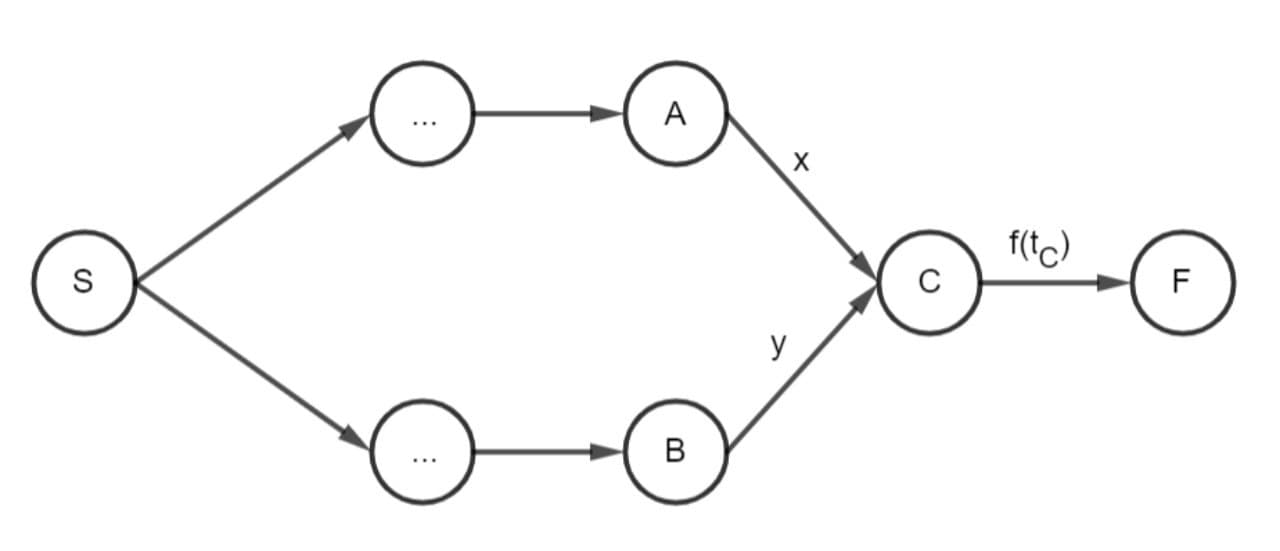
\includegraphics[scale=0.3]{graph_1.jpg}
\end{center}
\begin{center}
Рис 1.
\end{center}

Без ограничения общности, будем рассматривать часть маршрута P от точки C до F как одно ребро : C-F. Тогда обозначим время прохождения этого ребра как функцию $f(t_C)$, где $t_C$ - время старта из точки $C$. Вспомним неравенство прохождения для ребер (см. выше) : $f(t_a) \le (t_b - t_a) + f(t_b)$, где $\Delta = (t_b - t_a)$

Рассмотрим два маршрута $P : S-...-B-C-F$ и $P': S-...-A-C-F$.
Посчитаем время : $T(P) = t_b + f(t_b)$  и $T(P') = t_a + f(t_a)$
Используя неравенство, получаем : $T(P') = t_a + f(t_a) \le t_a + (t_b - t_a) + f(t_b) = T(P)$ Значит маршрут P не является минимальным. ЧТД


\newpage
\section*{Устойчивость нашего решения}



\newpage
\section*{Практические результаты}


\newpage
\section*{Сложность решения}

\newpage
\section*{Альтернативные подходы}

\newpage
\section*{Заключение}

\newpage
\section*{Список литературы}

\end{document}